\documentclass{article}
\usepackage{pgfplots}
\pgfplotsset{compat=1.16}

\begin{document}

\begin{figure}[ht]
    \centering
    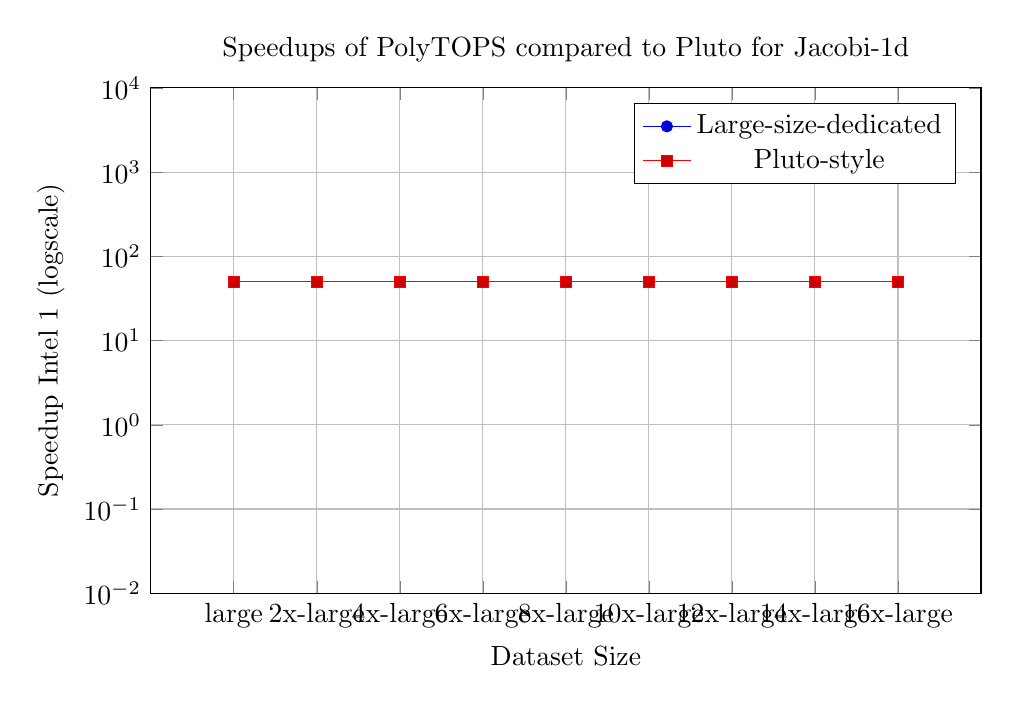
\begin{tikzpicture}
        \begin{axis}[
            width=\textwidth,
            height=8cm,
            xlabel={Dataset Size},
            ylabel={Speedup Intel 1 (logscale)},
            xmin=-1, xmax=9,
            ymin=-2, ymax=4,
            xtick={0,...,8},
            xticklabels={large, 2x-large, 4x-large, 6x-large, 8x-large, 10x-large, 12x-large, 14x-large, 16x-large},
            ytick={-2,-1,0,1,2,3,4},
            yticklabels={$10^{-2}$,$10^{-1}$,$10^{0}$,$10^{1}$,$10^{2}$,$10^{3}$,$10^{4}$},
            legend pos=north east,
            grid=major,
            log basis y={10},
            title={Speedups of PolyTOPS compared to Pluto for Jacobi-1d},
            ]
            \addplot coordinates {(0,24) (1,23.5) (2,22.5) (3,20.7) (4,19.2) (5,17.6) (6,15.6) (7,13.6) (8,11.7)};
            \addlegendentry{Large-size-dedicated};
            
            \addplot coordinates {(0,1.7) (1,1.7) (2,1.7) (3,1.7) (4,1.7) (5,1.7) (6,1.7) (7,1.7) (8,1.7)};
            \addlegendentry{Pluto-style};
        \end{axis}
    \end{tikzpicture}
    \caption{Speedups of PolyTOPS compared to Pluto for Jacobi-1d using two different configurations and multiple dataset sizes. The blue line represents the (best) dedicated configuration for large sizes, while the red line represents the Pluto-style configuration.}
    \label{fig:speedups_polytops_vs_pluto}
\end{figure}

\end{document}